\documentclass{beamer}
\newcommand{\myfont}{\rmfamily\normalsize\upshape\mdseries}
\newcommand{\degree}{^\circ}
\title{\sffamily Review V(Slides 269 - 330)}
\subtitle{\textbf{Master Theorem \& Partial Order}\\Good news! We're into TCS!}
\institute[UM-SJTU JI]{University of Michigan-Shanghai Jiao Tong University Joint Institute}
\author{HamHam}
\usepackage{graphicx}
\usepackage{picinpar}
\usepackage{indentfirst}
\usepackage{chemformula}
\usepackage{geometry}
\usepackage{subfigure}
\usepackage{appendix}
\usepackage{amsfonts}
\usepackage{enumerate}
\usepackage{float}
\usepackage{geometry}
\usepackage{latexsym}
\usepackage{listings}
\usepackage{multicol,multirow,multido}
\usepackage{tabularx}
\usepackage{ulem}
\usepackage{tikz}
\usepackage{xcolor}
\usepackage{cite}
\usepackage{setspace}
\usepackage{hyperref}
\usepackage{textpos}
\usepackage{booktabs}
\usepackage{diagbox}
\usepackage{listings}
\usepackage{graphics}
\usepackage{upgreek}
\usepackage{JI_MathCourse_Notations}
\usepackage{mathrsfs}
\usepackage[thicklines]{cancel}
%定义绘制椭圆的命令,带有四个参数
%第一个参数:椭圆位置的横坐标
%第二、三参数:椭圆x位置的半径、y位置的半径
%第四个参数:填充的透明度
\def\drawell#1#2#3#4{
	\draw[draw=black,fill=gray,fill opacity=#4,line width=3pt] 
	(#1,0) circle [x radius=#2, y radius=#3];}

%\usepackage{ctex} %插入中文
%\ctexset{today=old}

\newcommand{\mydef}[1]{\sffamily\blue{#1}\myfont\\} %for define
\newcommand{\mysol}{\yellow{Solution:}\\}
\usetheme[dove]{Boadilla}
\usecolortheme{dolphin}
\useoutertheme{miniframes}
\begin{document}
    \usebackgroundtemplate{\tikz\node[opacity=0.25]{
    \includegraphics[width=\paperwidth,
    height=\paperheight]{hamster.jpg}
    };}
\begin{titlepage}
    \begin{center}
        VE203 - Discrete Mathmatics 
    \end{center}
\end{titlepage}
\myfont
\newcommand{\binomial}[2]{\begin{pmatrix} {#1}\\{#2}	\end{pmatrix}}
\newcommand{\green}[1]{\textcolor[rgb]{0.3,0.6,0}{#1}}
\section{Asymptotic Notation}
\begin{frame}
    \frametitle{Asymptotic Notation}
    We define: 
    \begin{equation*}
        \begin{aligned}
            O\(g\(n\)\) &= \{f \(n\) \mid \exists c, n_0 \text{ s.t. }  0 \leq f\(n\) \leq c \cdot g\(n\), \text{ for } n \geq n_0\}\\
            \Omega \(g\(n\)\) & = \{f \(n\) \mid \exists c, n_0 \text{ s.t. }  0 \leq c \cdot g\(n\) \leq f\(n\), \text{ for } n \geq n_0\}\\
            \Theta \(g\(n\)\) & = O \(g\(n\)\) \cap \Omega \(g\(n\)\) \\
                              & = \{f\(n\) \mid \exists c_1,c_2,n_0 \text{ s.t. } c_1  g\(n\) \leq 
                              f\(n\) \leq c_2  g\(n\), \text{ for } n \geq n_0\}
        \end{aligned}
    \end{equation*}

    \vs{2em}
    \hh \yellow{Yep, this is the end of the story. I guess
     \green{$\omega(n)$} and \green{$o\(n\)$} won't appear
     in the exam.}
\end{frame}
\begin{frame}
    \frametitle{Exercise}
    1. Which of these symbols 
    $$ \Theta ~ O ~ \Omega ~ \xcancel{o ~ \omega} $$
    can go in these boxes? (List all that apply.)
    \begin{equation*}
        \begin{aligned}
            2n+\log n & = ~~~~~ (n) \\
            \log n    & = ~~~~~ (n) \\
            \sqrt{n}  & = ~~~~~ (\log _{300} n)\\
            n 2^n     & = ~~~~~ (n) \\
            n^7       & = ~~~~~ (1.01^n)
        \end{aligned}
    \end{equation*}
    % (Taken from \red{CCP 8.4})
\end{frame}
\begin{frame}
    \frametitle{Master Theorem}
    If $T\(n\) = aT\(n/b\) + f \(n\)$ (for constants $a \geq 1, b > 1$), then
    \begin{enumerate}
        \item $T \(n\) = \Theta (n^ {\log_b a})$ if $f\(n\) = O(n^{\log_b a-\varepsilon })$ for some constant $\varepsilon >0$
        \item $T \(n\) = \Theta (n^{\log_b a }\lg n)$ if $f\(n\)=\Theta \(n^{\log_b a}\)$
        \item $T \(n\) = \Theta \(f\(n\)\)$, if $f\(n\) = \Omega \(n^{\log_b a + \varepsilon}\)$
        for some constant $\varepsilon >0$ and regularity condition (\red{why?})
    \end{enumerate}
    \vv
    \textit{Comment.} This \green{would be provided} in the exam paper.
\end{frame}
\begin{frame}
    \frametitle{Exercise}
    2. Find the asymptotic bound for the following recurrence equations. Do you feel confused? \includegraphics[width=0.035\textwidth]{smile.png} 
    \begin{enumerate}
        \item  $$T\(n\) = 4 T\( \sqrt{n}\) + \log^5 n$$
        \item  $$T\(n\) =  T\( n / 2\)+ \lg n$$
    \end{enumerate}
    \begin{block}{Recipe}
        \begin{itemize}
            \item Compare $f\(n\)$ with  $n ^ {\log_b a}$
            \item Do substitution if necessary
        \end{itemize}
    \end{block}
    

\end{frame}
\begin{frame}
    \frametitle{Solution}

    Let $n=2^m$, i.e. $m = \log n$, then we have 
    $$ T(2^m) = 4 T(2^{m/2}) + m^5.$$
    Let $S(m) := T(2^m)$, then 
    $$S(m) = 4 S(m/2) + m^5, \quad f\(m\) = m^5$$ 
    By master theorem, $a = 4\geq 1, b =2 > 1, \log_b a =2$, so 
    $$S(m) = m^5  \in \Omega \(n^{\log_b a} + \varepsilon \) \text{~ for ~}  \varepsilon = 3,$$ 
    which is the case (iii) of the master 
    theorem, we have $S\(m\) = \Theta (m^5)$. 
    Substitue $n$ back, we have 
    $$T(n) = \Theta (\log ^5 n).$$
    

\end{frame}
\begin{frame}
    \frametitle{Solution ?}
    From Homework Ex 5.2
    \begin{itemize}
        \item If $f\(n\) = \Theta(n^{\log_b a} \log^k n)$ with $k \geq 0$, then $T(n) = \Theta(n^{\log_b a} \log ^{k+1} n)$.
    \end{itemize}
    \vv
    $$T(n) = T(n/2) + \lg n  \quad \Rightarrow \quad T(n) = \lg^2 n$$
    \begin{block}{Reference}
        \begin{itemize}
            \item MIT 6.024 Lecture Note: \url{http://people.csail.mit.edu/thies/6.046-web/master.pdf}
            \item Stanford cs161 Lecture Note Page 5: \url{https://web.stanford.edu/class/archive/cs/cs161/cs161.1168/lecture3.pdf}
            \item Online calculator: \url{https://www.wolframalpha.com/examples/mathematics/discrete-mathematics/recurrences}
        \end{itemize}
    \end{block}

\end{frame}
\section{Partial Order}
\begin{frame}
    \frametitle{Definition}
    \parbox{\textwidth}{
		\par A (binary) relation $R$ on $A$, \textit{i.e.,} $R \subset A \times A$, is
		\begin{itemize}
			\item[-] \textbf{ref\mbox{l}exive} if $aRa \Rightarrow \top$.
			\item[-] \textbf{symmetric} if $aRb \Leftrightarrow bRa$.
			\item[-] \textbf{transitive} if $aRb \wedge bRc \Rightarrow aRc$.
			\item[-] \textbf{anti-symmetric} if $aRb \wedge bRa \Rightarrow a = b$.
			\item[-] asymmetric if $aRb \wedge bRa \Rightarrow \perp$.
			\item[-] total if $aRb \vee bRa \Rightarrow \top$.
		\end{itemize}
		\par \phantom{ji}
		\par \textbf{(Non-strict) Partial order}: reflexive, antisymmetric, and transitive.
		\par \textbf{Equivalence relation}: reflexive, symmetric, and transitive.
        \par \textbf{Total order:} Partial order + total.
    }
\end{frame}
\begin{frame}
    \frametitle{Partial Order}
    \fbox{
	\parbox{0.95\textwidth}{
    \hh The term partial order typically refers to a \textbf{non-strict} 
    partial order relation.
	\par \phantom{ji}\\
	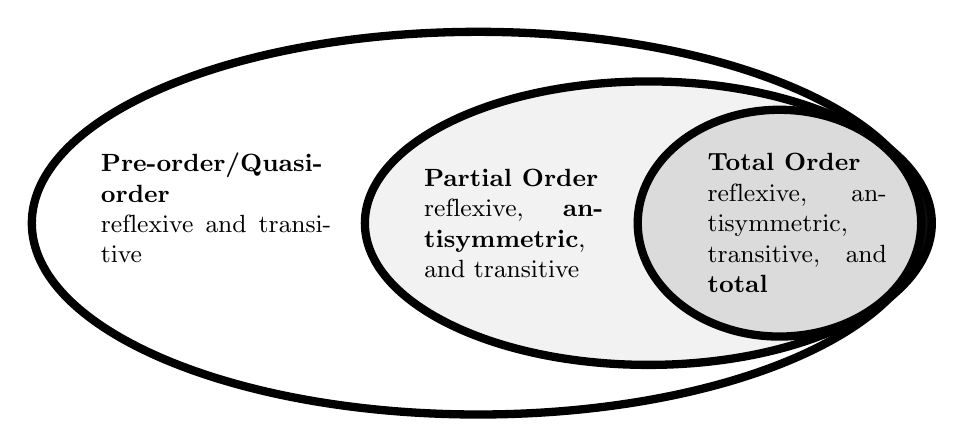
\begin{tikzpicture}[font=\rmfamily\small,scale=.9]
	\drawell{-1}{6.3}{2.7}{0};
	%标记节点,添加文字
	%使用垂直盒子,规定盒子宽度与对齐方式
	\node at (-4.7,0) {\parbox[c]{9em}{\textbf{Pre-order/Quasi-order}\\
			ref\mbox{l}exive and transitive\\}};
	%前两个参数之和为8,才能保证三个椭圆相切于右端点
	\drawell{1.4}{4}{2}{.1};
	\node at (-0.5,0) {\parbox[c]{7em}{\textbf{Partial Order}\\
			ref\mbox{l}exive, \textbf{antisymmetric}, and transitive}};
	
	\drawell{3.25}{2}{1.6}{.2};
	\node at (3.5,0) {\parbox[c]{7em}{\textbf{Total Order}\\
			ref\mbox{l}exive, antisymmetric, transitive, and \textbf{total}}};
	\end{tikzpicture}
	}
}
\end{frame}
\begin{frame}
    \frametitle{Concept Checking List}
    Be familiar with the following:
    \begin{itemize}
        \item covers/adjacent
        \item minimal/minimum element
        \item maximal/maximum element
        \item (in)comparability graph
        \item chain/antichain
        \item \sout{lattice: join and meet}
    \end{itemize}
    \vv
    \red{\large{Let's see one example!}}
\end{frame}
\begin{frame}
    \frametitle{Example}
    \fbox{
	\parbox{0.95\textwidth}{
	 	\hh Hasse/Order Diagram: edges are the \textbf{\green{cover}} pairs $(x, y)$ with $x$ covered by $y$.
	 	\par \phantom{ji}\\
	 	\centering
	 	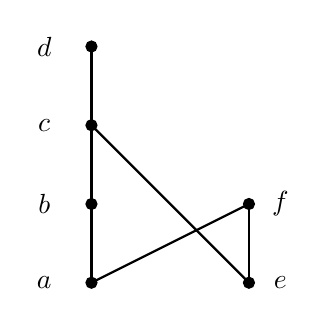
\begin{tikzpicture}
	 	%% vertices
	 	\draw[fill=black] (9,0) circle (2pt);
	 	\draw[fill=black] (9,1) circle (2pt);
	 	\draw[fill=black] (7,0) circle (2pt);
	 	\draw[fill=black] (7,1) circle (2pt);
	 	\draw[fill=black] (7,2) circle (2pt);
	 	\draw[fill=black] (7,3) circle (2pt);
	 	%% vertex labels
	 	\node at (6.4,0) {$a$};
	 	\node at (6.4,1) {$b$};
	 	\node at (6.4,2) {$c$};
	 	\node at (6.4,3) {$d$};
	 	\node at (9.4,0) {$e$};
	 	\node at (9.4,1) {$f$};
	 	%%% edges
	 	\draw[thick] (9,0) -- (9,1);
	 	\draw[thick] (7,0) -- (7,1) -- (7,2) -- (7,3);
	 	\draw[thick] (9,0) -- (7,2);
	 	\draw[thick] (7,0) -- (9,1);
	 	\end{tikzpicture}
	}
}
    \begin{block}{Question}
        \hh Fill in CCP03: ex2-ex5. Do be careful!
    \end{block}
\end{frame}
\begin{frame}
    \frametitle{Exercise}
    3. In the poset $(\mathbb{Z}^+, \mid)$ (where $\mathbb{Z}^+$ is the set of 
    all positive integers and $\mid$ is the divides relation), are the integers 3 and 9 comparable? 
    Are 7 and 10 comparable? \\
    \vs{2em}
    \pause
    \yellow{Solution:}\\
    \hh 3 and 9 are comparable since $3 \mid 9$, \textit{i.e.}, 
    3 divides 9. But 7 and 10 are not comparable since $7 \nmid 10$  
    and $10 \nmid 7$. 
\end{frame}
\begin{frame}
    \frametitle{Exercise}
    4.  A relation $R$ is defined on ordered pairs of integers as follows: $(x,y) R(u,v)$ if $x < u$ and $y > v$. Then $R$ is:
    \begin{enumerate}[(A)]
        \item Neither a partial order nor an equivalence relation
        \item A partial order but not a total order
        \item A total order
        \item An equivalence relation
    \end{enumerate}
    \vs{2em}
    \yellow{Answer:} A
\end{frame}
\begin{frame}
    \frametitle{Exercise}
    5. Given a set $S=\{a, b, c, d\} .$ Consider the following 4 partitions 
    $\pi_{1}, \pi_{2}, \pi_{3}, \pi_{4}$ on $S$: 
    \begin{center}
        $\pi_{1}=\{\overline{a b c d}\}, \pi_{2}=\{\overline{a b}, \overline{c d}\}, \pi_{3}=\{\overline{a b c}, \bar{d}\}, \pi_{4}=\{\bar{a}, \bar{b}, \bar{c}, \bar{d}\} .$ \\
    \end{center}
    \hh Let $p$ be a \textbf{strict} partial order on the set of partitions $S^{\prime}=\left\{\pi_{1}, \pi_{2}, \pi_{3}, \pi_{4}\right\}$ defined as follows: 
    \begin{center}
        $\pi_{i} p \pi_{j}$ if and only if $\pi_{i}$ refines $\pi_{j}$\\ 
    \end{center}
    \hh Find the poset diagram for $\left(S^{\prime}, p\right)$. 
\end{frame}
\begin{frame}
    \frametitle{Solution}
    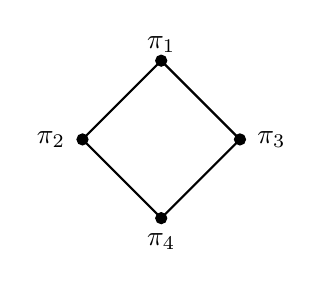
\begin{tikzpicture}
        % vertices
        \draw[fill=black] (0,1) circle (2pt);
        \draw[fill=black] (1,0) circle (2pt);
        \draw[fill=black] (1,2) circle (2pt);
        \draw[fill=black] (2,1) circle (2pt);
        % vertex labels
        \node at (-0.4,1) {$\pi_{2}$};
        \node at (1,-0.3) {$\pi_{4}$};
        \node at (1,2.2) {$\pi_{1}$};
        \node at (2.4,1) {$\pi_{3}$};
        % edges
        \draw[thick] (0,1) -- (1,0) -- (2,1) -- (1,2) -- (0,1);
        \end{tikzpicture}
        \\\hh A partition is said to refine another partition if it splits the sets 
        in the second partition to a larger number of sets.
        \\\hh Therefore, the partial order contains the following ordered pairs: 
        $$\{(\pi_4,\pi_1),(\pi_4,\pi_2),(\pi_4,\pi_3),(\pi_3,\pi_1),(\pi_2,\pi_1)\}$$        
\end{frame}

\section{End}
\begin{frame}
    \frametitle{Reference}

    \begin{itemize}
        \item Homework exercises from 2023-Summer-Ve203
        \item Exercises/graphics from 2021-Fall-Ve203 TA Zhao Jiayuan
    \end{itemize}

\end{frame}
\begin{frame}
    \centering
    \Huge{$\mathcal{THANKS}$!}
\end{frame}

\end{document}